\documentclass[../../main/main.tex]{subfiles}
\begin{document}
\section{Game Value}
\label{sec:game_value}

Having characterized the Nash equilibrium strategy profile in Section 4, we now turn to analyzing the expected payoff when both players employ these optimal strategies. In zero-sum games like Limit Continuous Poker, the concept of game value is fundamental. The game value represents the expected payoff that the first player (bettor) can guarantee when both players play optimally. Since this is a zero-sum game, the caller's expected payoff is simply the negative of this value. This value serves as a measure of how favorable the game is to the bettor under the given betting limits $L$ and $U$.

\begin{theorem}
    \label{thm:game_value}
    The value of Limit Continuous Poker is given by:
    \[
        V_{LCP}(L, U) = \frac{(1 + L)^3(1+U)^3 - ((1+L)^3+L^3(1 + U)^3)}{14(1 + L)^3(1+U)^3 - 2((1+L)^3+L^3(1 + U)^3)}
    \]
    Equivalently, using the change of variables $r = L/(1+L)$ and $t = 1/(1+U)$, this can be written more compactly as:
    \[
        V(r, t) = \frac{1 - r^3 - t^3}{14 - 2r^3 - 2t^3}
    \]
\end{theorem}

\begin{customproof}
    Since LCP is a zero-sum game, all Nash equilibria yield the same payoff. We have explicitly constructed optimal strategies for both players, so the value of the game is the expected payoff of these strategies, averaged over all hand pairs $(x, y)$. This reduces to an integral of the payoff over the unit square, like we saw in Figure \ref{fig:payoffs}. 
    
    The computation is extremely nontrivial because the bet size is only defined implicitly in terms of the hand strength $x$. The proof requires breaking the unit square into regions based on the strategies and bet sizes, then computing the expected value as a weighted sum of payoffs over these regions. The full technical details are provided in Appendix \ref{sec:value_computation}.
\end{customproof}

This is a rational function of $L$ and $U$ with a surprisingly simple form. The change of variables to $r$ and $t$ reveals an even more elegant structure, along with the following symmetry property:

\begin{align*}
    V_{LCP}(L, U) &= V_{LCP}\left(\frac{1}{U}, \frac{1}{L}\right)\\
    \text{or equivalently, } V(r, t) &= V(t, r)
\end{align*}

The symmetry becomes immediately apparent in the $(r,t)$ formulation: the numerator $1 - r^3 - t^3$ and denominator $14 - 2r^3 - 2t^3$ are both symmetric in $r$ and $t$. This is not at all obvious from the game setup in terms of $L$ and $U$.

Figure \ref{fig:game_value_rt} shows the game value as a function of $r$ and $t$, making the symmetry $V(r,t) = V(t,r)$ visually apparent as a reflection across the diagonal. The plot also clearly illustrates the interpretations discussed above: the left edge ($r=0$, corresponding to $L=0$) represents the case where minimum bets are negligible, while the bottom edge ($t=0$, corresponding to $U \to \infty$) represents the case where maximum bets become arbitrarily large. The diagonal ($r+t=1$, or equivalently $L=U$) represents the boundary where the game reduces to fixed-bet continuous poker.

In terms of the original parameters, the symmetry $V_{LCP}(L, U) = V_{LCP}(1/U, 1/L)$ tells us that the benefit from increasing $U$ is exactly equivalent to that of decreasing $L$ in a reciprocal manner, centered around the pot size of $1$. For example, suppose you are given the choice between playing LCP as the bettor with limits $L=1/2$ and $U=5$ or $L=1/5$ and $U=2$. You know you can play optimally, but it is unclear which game favors you. The symmetry property tells us that the value of the game is the same in both cases, so you should be indifferent between the two.

\begin{figure}[h!]
    \centering
    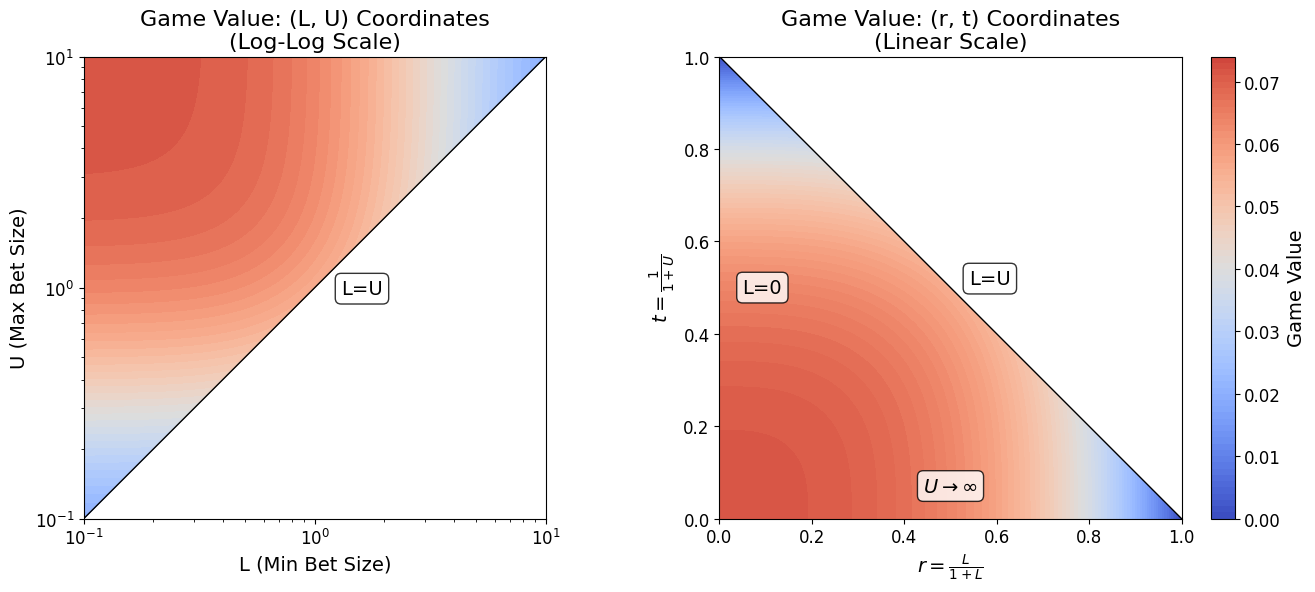
\includegraphics[width=1.1\textwidth]{images/game_value_plots.png}
    \caption{Game value as a function of both parametrizations. The symmetry about the diagonal is immediately visible, corresponding to $V(r,t) = V(t,r)$ or $V(L, U) = V(1/U, 1/L)$. Note that the left plot is cutting off extremely large and small values of $L$ and $U$, while the right plot shows every possible parameter combination.}
    \label{fig:game_value_fig}
\end{figure}

\subsection{Interpreting the Parameters r and t}

Before analyzing the properties of the game value, it is helpful to understand what the transformed parameters $r$ and $t$ represent in game-theoretic terms.

\textbf{The parameter $r = L/(1+L)$ as minimum pot odds:}
When the bettor makes a minimum bet of size $L$, the pot grows from 1 to $1+L$. The caller must risk $L$ to call and potentially win a pot of $1+L$. Thus, $r = L/(1+L)$ represents the \emph{pot odds} the caller receives when facing a minimum bet---the ratio of what they risk to the total pot. This is the most favorable pot odds any caller ever faces in LCP, since larger bets offer worse pot odds. As $L \to 0$, we have $r \to 0$, meaning the minimum bet becomes negligible and calling becomes essentially free. As $L \to \infty$, we have $r \to 1$, meaning the minimum bet becomes prohibitively expensive relative to the pot.

\textbf{The parameter $t = 1/(1+U)$ as pot fraction at maximum bet:}
When the bettor makes a maximum bet of size $U$, the pot grows from 1 to $1+U$. The parameter $t = 1/(1+U)$ represents the original pot as a fraction of the total pot after a maximum bet. Equivalently, $1-t = U/(1+U)$ represents the pot odds the caller receives when facing a maximum bet. A small value of $t$ (close to 0) indicates that $U$ is very large relative to the pot, allowing the bettor to make very aggressive bets. As $U \to \infty$, we have $t \to 0$, meaning the maximum bet becomes arbitrarily large. As $U \to 0$, we have $t \to 1$, meaning the maximum bet becomes negligible.

\textbf{The duality revealed by the symmetry:}
The parameter $r$ fundamentally controls the \emph{caller's incentive to call} with marginal hands: higher $r$ means the minimum bet offers worse pot odds, discouraging calls. The parameter $t$ fundamentally controls the \emph{bettor's ability to apply pressure}: lower $t$ means the maximum bet can be much larger relative to the pot, allowing more aggressive play. The symmetry $V(r,t) = V(t,r)$ reveals a deep duality in the game: swapping the ``minimum calling incentive'' (measured by $r$) with the ``maximum betting freedom'' (measured inversely by $t$) produces games with identical value. This is remarkable because $r$ is primarily about the caller's decisions (pot odds when facing small bets) while $t$ is primarily about the bettor's decisions (how large they can bet), yet these two forces are perfectly balanced in determining the game's value.

In the following sections, we investigate the properties and behavior of $V_{LCP}(L, U)$ in more detail. These include monotonicity, convergence to NLCP and FBCP, and the symmetry property.


\subsection{Value Monotonicity}

Intuitively, more options for the bettor should increase the game's value. Notice the higher value for more lenient limits (red regions of Figure \ref{fig:game_value_fig}) and lower value for more strict limits (blue corners). We can easily prove this formally:

\begin{theorem}
    The value of Limit Continuous Poker is weakly monotonically increasing in $U$ and weakly monotonically decreasing in $L$:
\[
    \frac{\partial V_{LCP}(L, U)}{\partial U} \geq 0, \;\; \frac{\partial V_{LCP}(L, U)}{\partial L} \leq 0.
\]
\end{theorem}
\begin{customproof}
    We can express the derivatives in terms of the cleaner $(r,t)$ variables. Since $r = L/(1+L)$ and $t = 1/(1+U)$, we have:
    \begin{align*}
        \frac{dr}{dL} = \frac{1}{(1+L)^2}, \quad \frac{dt}{dU} = -\frac{1}{(1+U)^2}
    \end{align*}

    Using the chain rule and the fact that $V(r,t) = \frac{1-r^3-t^3}{14-2r^3-2t^3}$:
    \begin{align*}
        \frac{\partial V}{\partial r} &= \frac{-3r^2(14-2r^3-2t^3) + 2 \cdot 3r^2(1-r^3-t^3)}{(14-2r^3-2t^3)^2} = \frac{-18r^2(2-r^3-t^3)}{(14-2r^3-2t^3)^2} < 0\\
        \frac{\partial V}{\partial t} &= \frac{-18t^2(2-r^3-t^3)}{(14-2r^3-2t^3)^2} < 0
    \end{align*}

    where the inequalities hold since $r, t \in (0,1)$ implies $r^3 + t^3 < 2$ and $14 - 2r^3 - 2t^3 > 0$. Therefore:
    \begin{align*}
        \frac{\partial V_{LCP}}{\partial L} &= \frac{\partial V}{\partial r} \frac{dr}{dL} = \frac{-18r^2(2-r^3-t^3)}{(14-2r^3-2t^3)^2} \cdot \frac{1}{(1+L)^2} < 0 \\
        \frac{\partial V_{LCP}}{\partial U} &= \frac{\partial V}{\partial t} \frac{dt}{dU} = \frac{-18t^2(2-r^3-t^3)}{(14-2r^3-2t^3)^2} \cdot \left(-\frac{1}{(1+U)^2}\right) > 0
    \end{align*}
\end{customproof}

\subsection{Value Convergence}

The main diagonal of the plots in Figure \ref{fig:payoffs_vs_LU_combined} should represent $L=U$, which means the bet size is fixed. Thus, this diagonal should represent the value of FBCP for various values of $B$. We can prove this formally:

\begin{theorem}
    For any $B > 0$, the value of Limit Continuous Poker converges to the value of Fixed-Bet Continuous Poker as $L$ and $U$ approach $B$:
\[
\lim_{L \to B} \lim_{U \to B} V_{LCP}(L, U) = \lim_{U \to B} \lim_{L \to B} V_{LCP}(L, U) = V_{FB}(B)
\]
\end{theorem}

\begin{customproof}
    $V_{LCP}(L, U)$ is a rational function of $L$ and $U$, and no part of the expression is undefined for $L = U = B$. We can simply plug in and simplify to get
    $$ \frac{B}{2(1+2B)(2+B)}, $$
    which is exactly $V_{FB}(B)$.
\end{customproof}

These plots also align with the known result that a fixed pot-size bet of $B=1$ maximizes the expected value for the bettor in FBCP, as seen by the fact that $(1, 1)$ achieves the maximum value on the diagonal. 

We can also show that the value of LCP converges to the value of NLCP as $L$ and $U$ approach their extremes, represented by the top left of any plot in Figure \ref{fig:payoffs_vs_LU_combined}.

\begin{theorem}
    The value of Limit Continuous Poker converges to the value of NLCP as $L$ and $U$ approach $0$ and $\infty$:
\[
\lim_{L \to 0} \lim_{U \to \infty} V_{LCP}(L, U) = \lim_{U \to \infty} \lim_{L \to 0} V_{LCP}(L, U) = V_{NL}
\]
\end{theorem}
\begin{customproof}
    We can simply plug in $L=0$ to get
    $$\frac{(U+1)^3-1}{14 (U+1)^3-2}.$$
    Taking the limit as $U \to \infty$ gives $\frac{1}{14} = V_{NL}$.
\end{customproof}

\end{document}